\documentclass{article}
\usepackage[T1]{fontenc}
\usepackage{lmodern}
\usepackage{graphicx}
\usepackage{amsmath,amssymb}
\usepackage[a4paper,margin=2cm]{geometry}
\usepackage[absolute,overlay]{textpos}
\setlength{\TPHorizModule}{1mm}
\setlength{\TPVertModule}{1mm}
\usepackage[indonesian]{babel}
\usepackage{hyperref}
\setlength{\emergencystretch}{2em}
% unit: Halaman 22

\begin{document}

% === Halaman 22 (llm) ===

\begin{itemize}
    \item Kebocoran data di Kemenhan dan Bank BSI
\end{itemize}

\vspace{5mm}

\begin{center}
    \textbf{KEJAHATAN SIBER}\\
    \Huge \textbf{Situs Kementerian Pertahanan Diduga Diretas, Dokumen Rahasia Berpotensi Bocor}\\
    Data Kementerian Pertahanan sebesar 1,64 terabita berpotensi bocor setelah situs resmi kementerian itu dibobol peretas.
\end{center}

\vspace{10mm}

\begin{center}
    \huge \textbf{1,5 TB Data Nasabah BSI Dibobol Hacker LockBit 3.0}\\
    \small Taufan Bara Mukti $\square$ Sabtu, 13 Mei 2023 | 12:03 WIB
\end{center}

% deskripsi: Foto gedung Bank Syariah Indonesia (BSI) sebagai ilustrasi berita kebocoran data.
% bbox normalisasi: [0.2070, 0.7030, 0.7200, 1.0000]
\begin{textblock*}{107.73mm}(43.47mm,208.79mm)
\noindent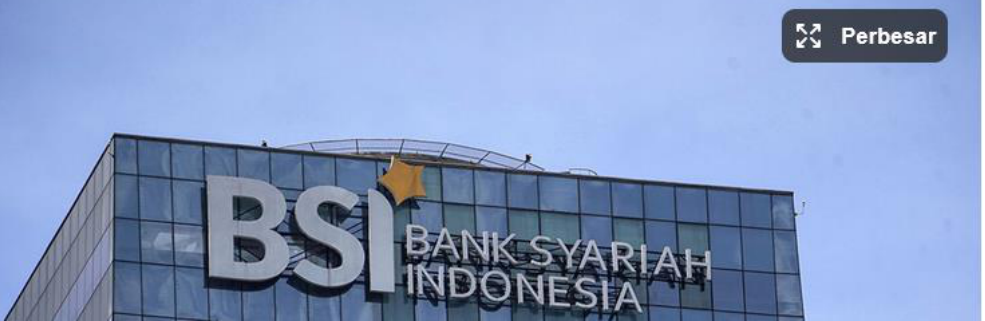
\includegraphics[width=107.73mm,height=88.21mm]{../../images/llm/page_022_img_01.png}%
\end{textblock*}

\end{document}
